\subsection{Bragg Bedingung}
Zur Überprüfung der Bragg Bedingung wird der LiF-Kristall auf einen Winkel von $\theta = 14°$ gestellt.
Das Geiger-Müller Zählrohr rotiert um den Kristall von $\alpha_{\text{Z}} = 26° - 30°$ Grad in $\Delta\alpha = 0,1°$ Schritten.
Die gemessenen Daten sind in der Tabelle \ref{tab:bragg} zu finden. Die Tabelle ist in der Graphik \ref{fig:bragg} dargestellt.\\
Den Daten lässt sich ein Maximum für $\alpha_{\text{Z}} = 28°\pm 0,2°$ entnehmen.
\begin{figure}[h!]
  \centering
  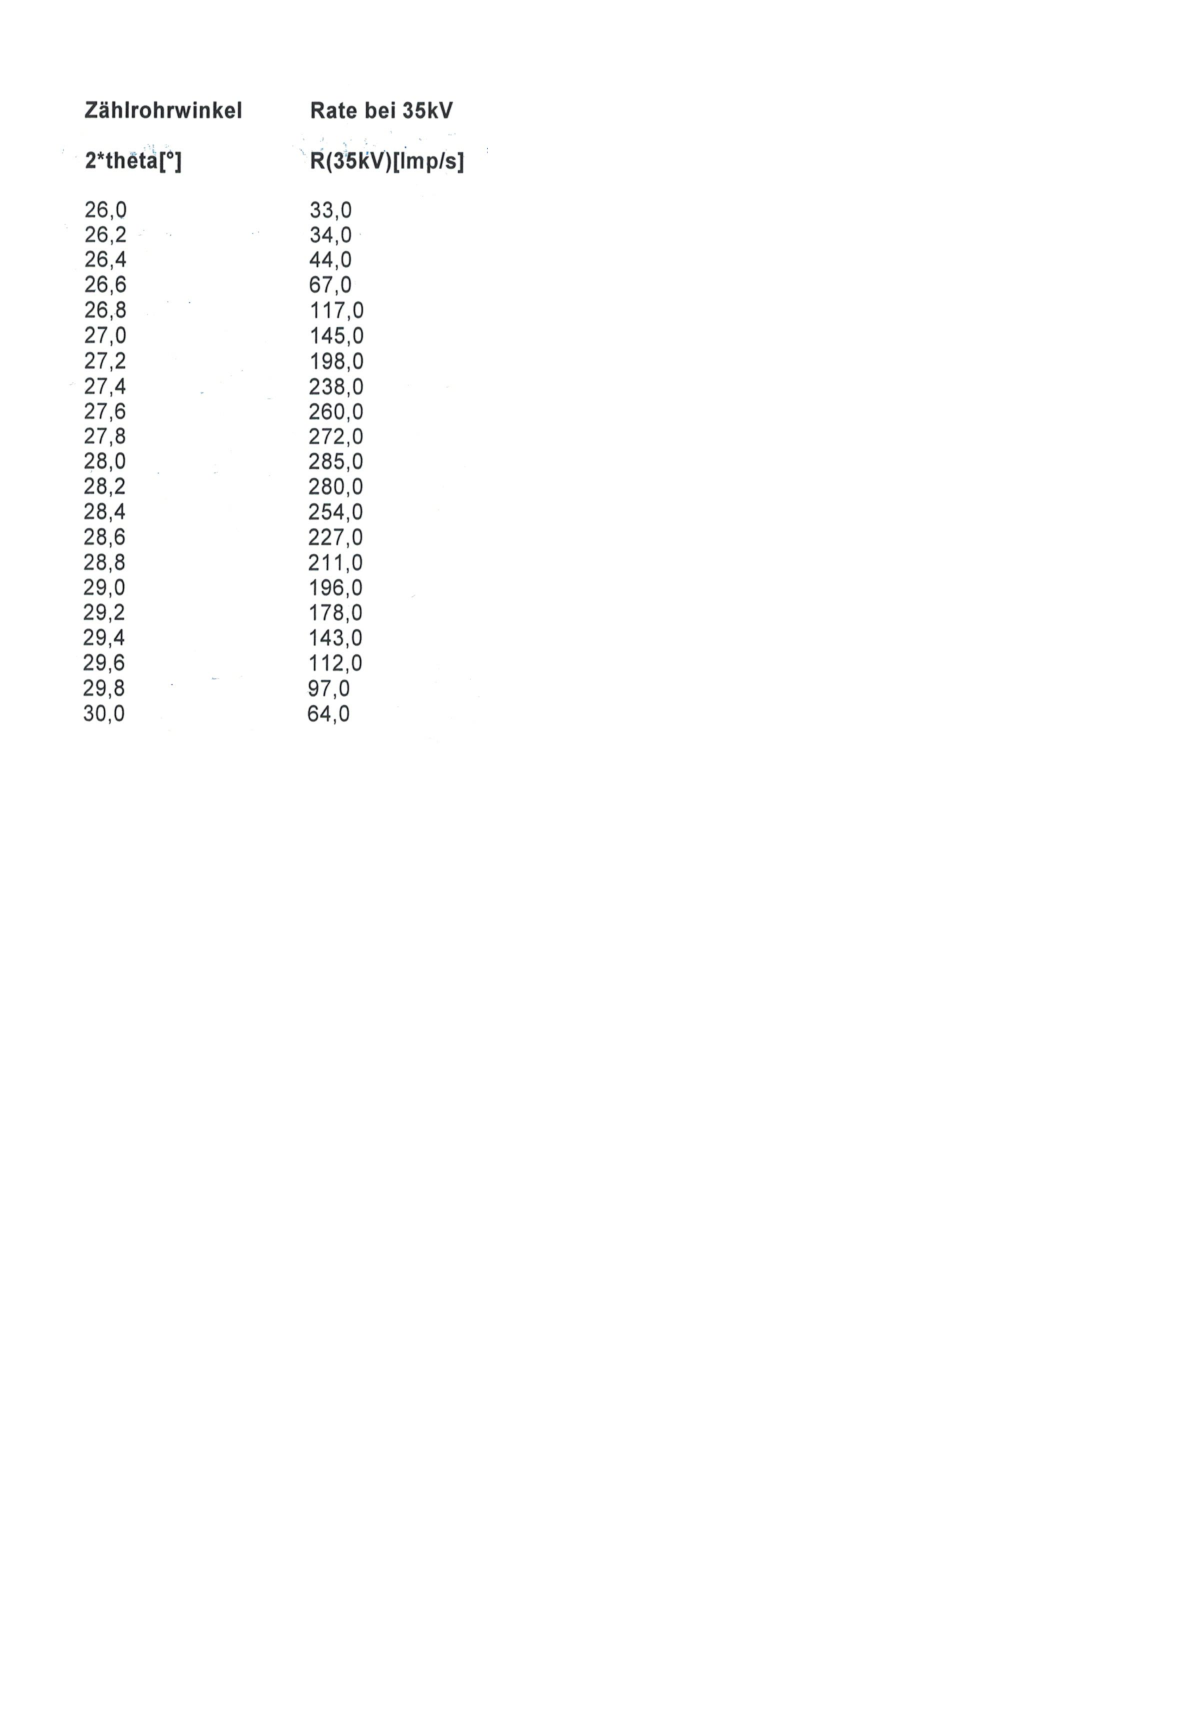
\includegraphics[width=0.4\textwidth]{braggtab.pdf}
  \caption{Messwerte zur Überprüfung der Bragg Bedingung}
  \label{tab:bragg}
\end{figure}
\begin{figure}[h!]
  \centering
  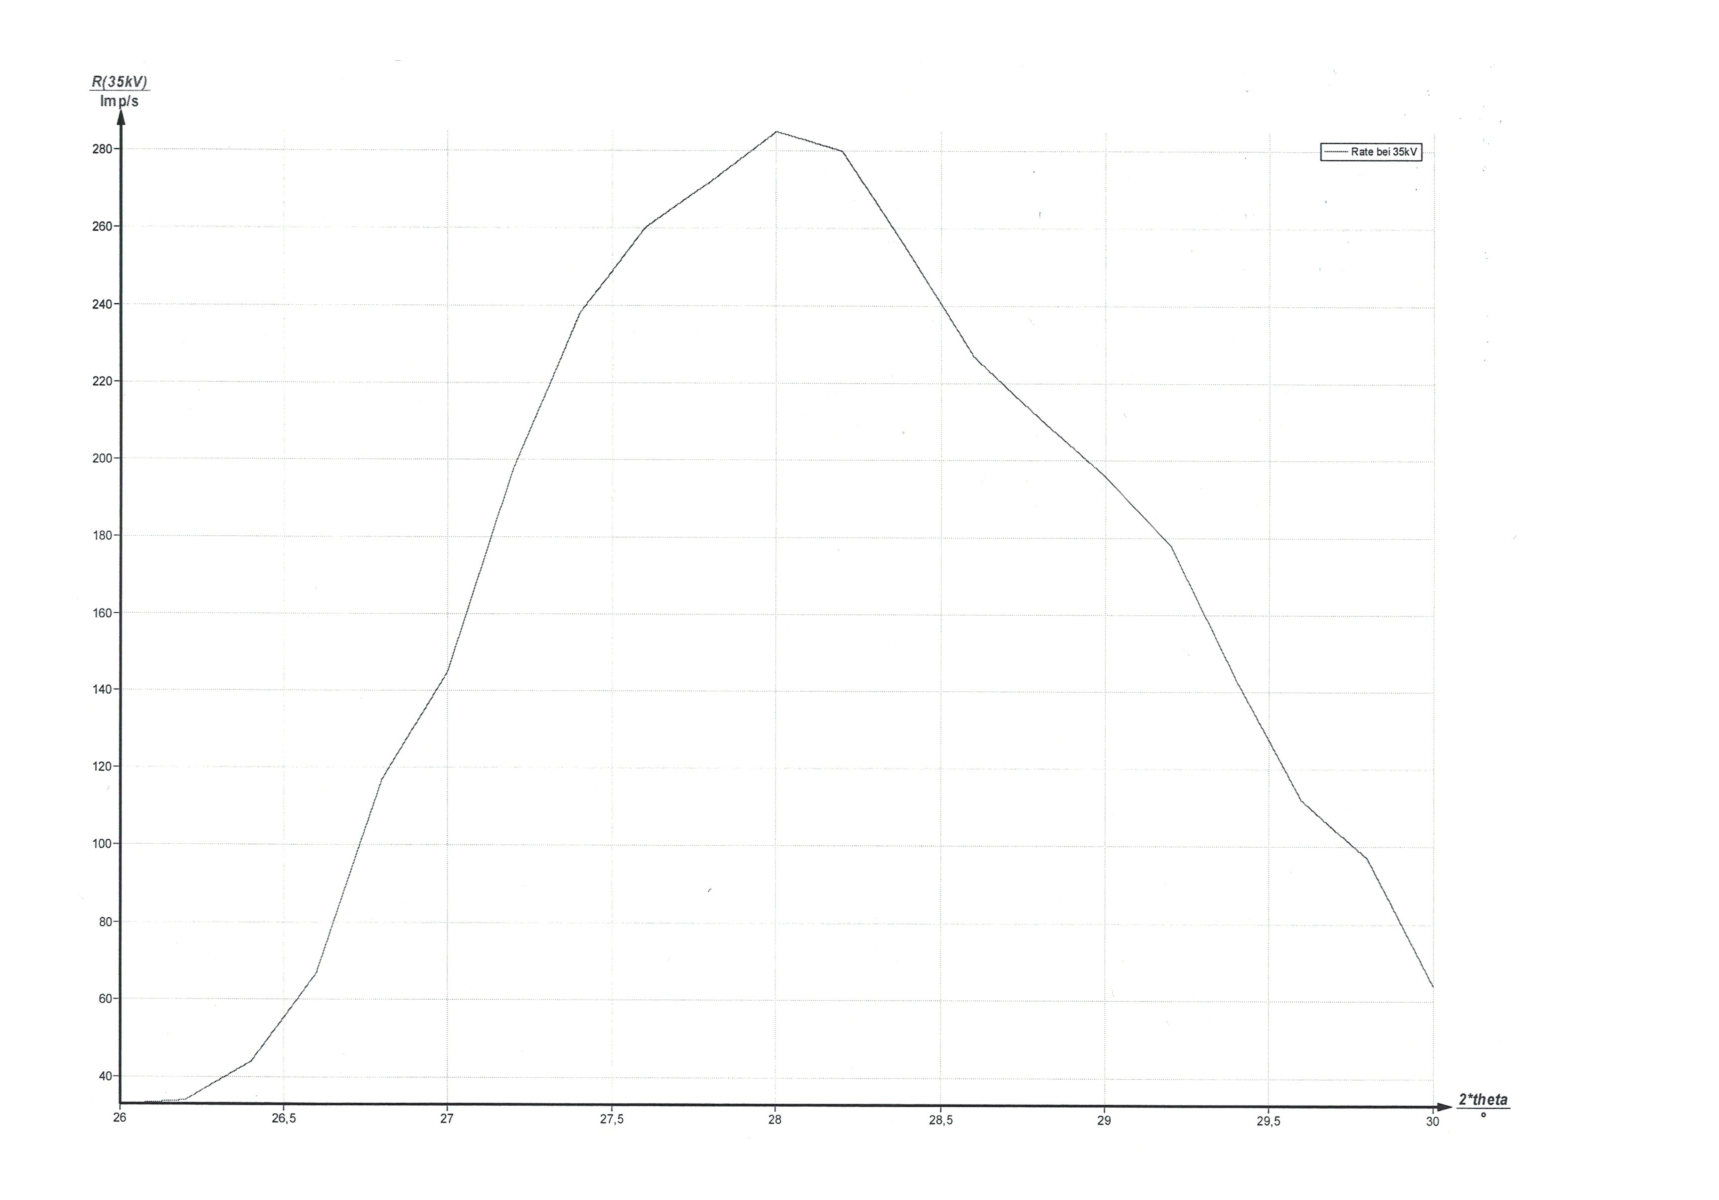
\includegraphics[width=\textwidth]{bragggraph.pdf}
  \caption{Überprüfung des Bragg-Winkels}
  \label{fig:bragg}
\end{figure}
\FloatBarrier
\subsection{Emissionsspektrum einer Cu-Röntgenröhre}
Um das Emissionsspektrum der Cu-Röntgenröhre zu vermessen wird der Kristall von $\theta = 4° - 26°$ gedreht.
Das Geiger-Müller Zählrohr wird wegen der Bragg Bedingung auf den doppelten Winkel eingestellt.
Die gemessenen Daten sind in der Tabelle \ref{tab:emiss} aufgefürt.
Die Messdaten sind in der Graphik \ref{fig:emiss} dargestellt.
Der Winkel der $K_{\text{$\beta$}}$ Linie und der $K_{\text{$\alpha$}}$ Linie werden abgelesen. Daraus werden die
Werte für die Wellenlänge und die Energie berechnet.
\begin{align*}
  K_{\text{$\beta$}}&                                          &K_{\text{$\alpha$}}&\\
  \theta_{\text{$\beta$}} &= \SI{20\pm 0,2}°                   &\theta_{\text{$\alpha$}} &= \SI{22,4\pm 0,2}°\\
  \lambda_{\text{$\beta$}} &= \SI{0,1377\pm0,0013}{nm}         &\lambda_{\text{$\alpha$}} &= \SI{0,1535\pm0,0013}{nm}\\
  E_{\text{$\beta$}} &= \SI{9,00\pm0,08}{keV}                     &E_{\text{$\alpha$}} &= \SI{8,077\pm0,06}{keV}
\end{align*}
Die Wellenlänge berechnet sich nach der Gleichung \ref{eqn:lambda}.
\\Der Grenzwinkel, welcher die kleinste Wellenlänge besitzt und somit die größte Energie, kann an der Graphik \ref{fig:emiss} abgelesen werden.
\begin{align*}
    &\theta_{1} = \SI{4,8\pm0,2}°\\
    &\lambda = \SI{0,0337\pm0,0014}{nm}\\
    &E_{\text{max}}=\SI{36,784\pm1,468}{keV}
\end{align*}
Die Halbwertsbreite der $K_{\text{$\beta$}}$ Linie und der $K_{\text{$\alpha$}}$ Linie wird gemessen,
 in dem man ermittelt bei welchem Winkel die Intensität um die Hälfte abgefallen ist.
 Über die Gleichungen \ref{eqn:winkel} und \ref{eqn:lambda} lässt sich für den Winkel die Energie ausrechnen.
\begin{align*}
    &K_{\text{$\beta$}}         &K_{\text{$\alpha$}}\\
    &\theta_{1} = \SI{19,7\pm0,2}{°}   &\theta_{1} &= \SI{22,2\pm0,2}{°}\\
    &\theta_{2} = \SI{20,3\pm0,2}{°}    &\theta_{2} &=\SI{22,6\pm0,2}{°}\\
    &E_{1} = \SI{9,131\pm0,088}{keV}     &E_{1} &= \SI{8,146\pm0,069}{keV}\\
    &E_{2} = \SI{8,872\pm0,082}{keV}     &E_{2} &= \SI{8,009\pm0,066}{keV}
\end{align*}


Mit den Gleichungen \ref{eqn:E} und \ref{eqn:E2} lässt sich für $K_{\text{$\beta$}}$ und $K_{\text{$\alpha$}}$,
die Abschirmkonstante $\sigma_{\text{K}}$ bestimmen.
\begin{align*}
  \sigma_{\text{$K_{\beta}$}}&=\SI{3,28\pm0,12}{}\\
  \sigma_{\text{$K_{\alpha}$}}&=\SI{12,53\pm0,54}{}
\end{align*}


\begin{figure}[h!]
  \centering
  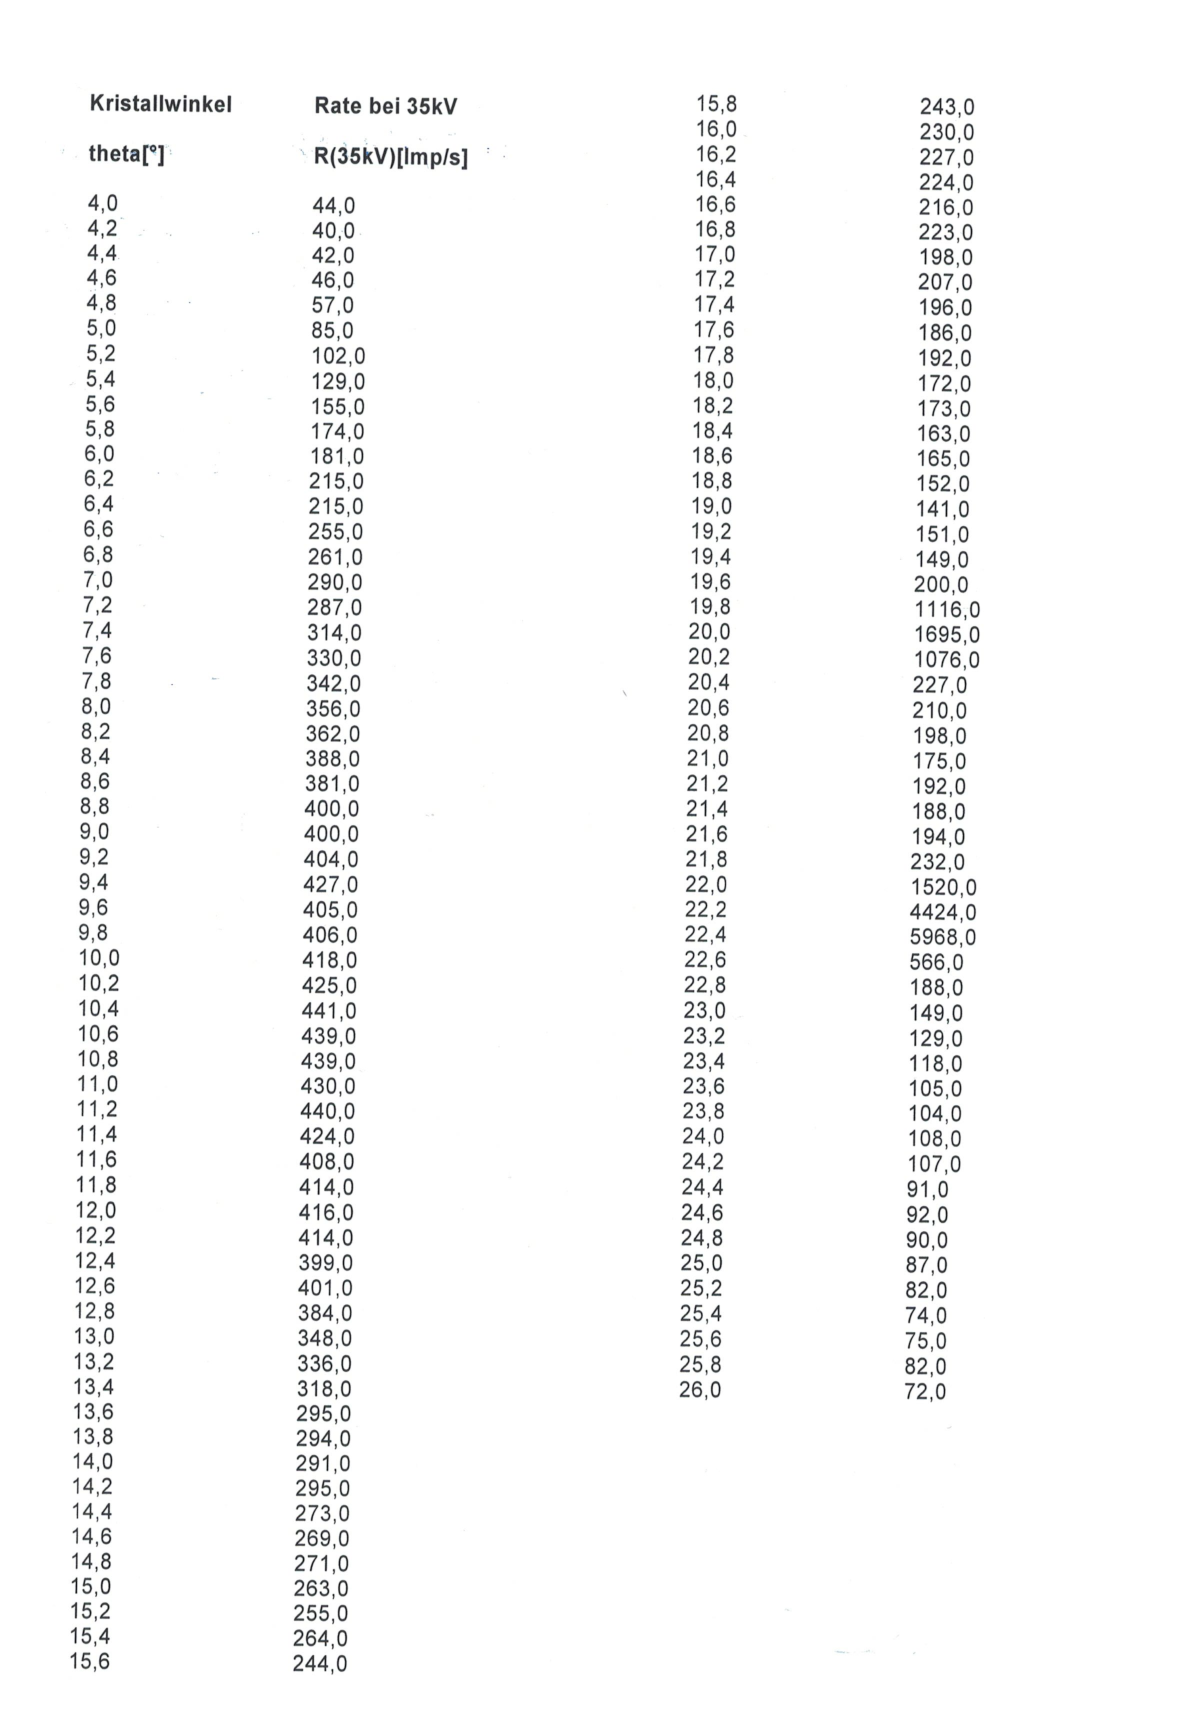
\includegraphics[width=0.8\textwidth]{emissiontab.pdf}
  \caption{Tabelle zum Emissionsspektrum einer Cu-Röntgenröhre}
  \label{tab:emiss}
\end{figure}
\begin{figure}[h!]
  \centering
  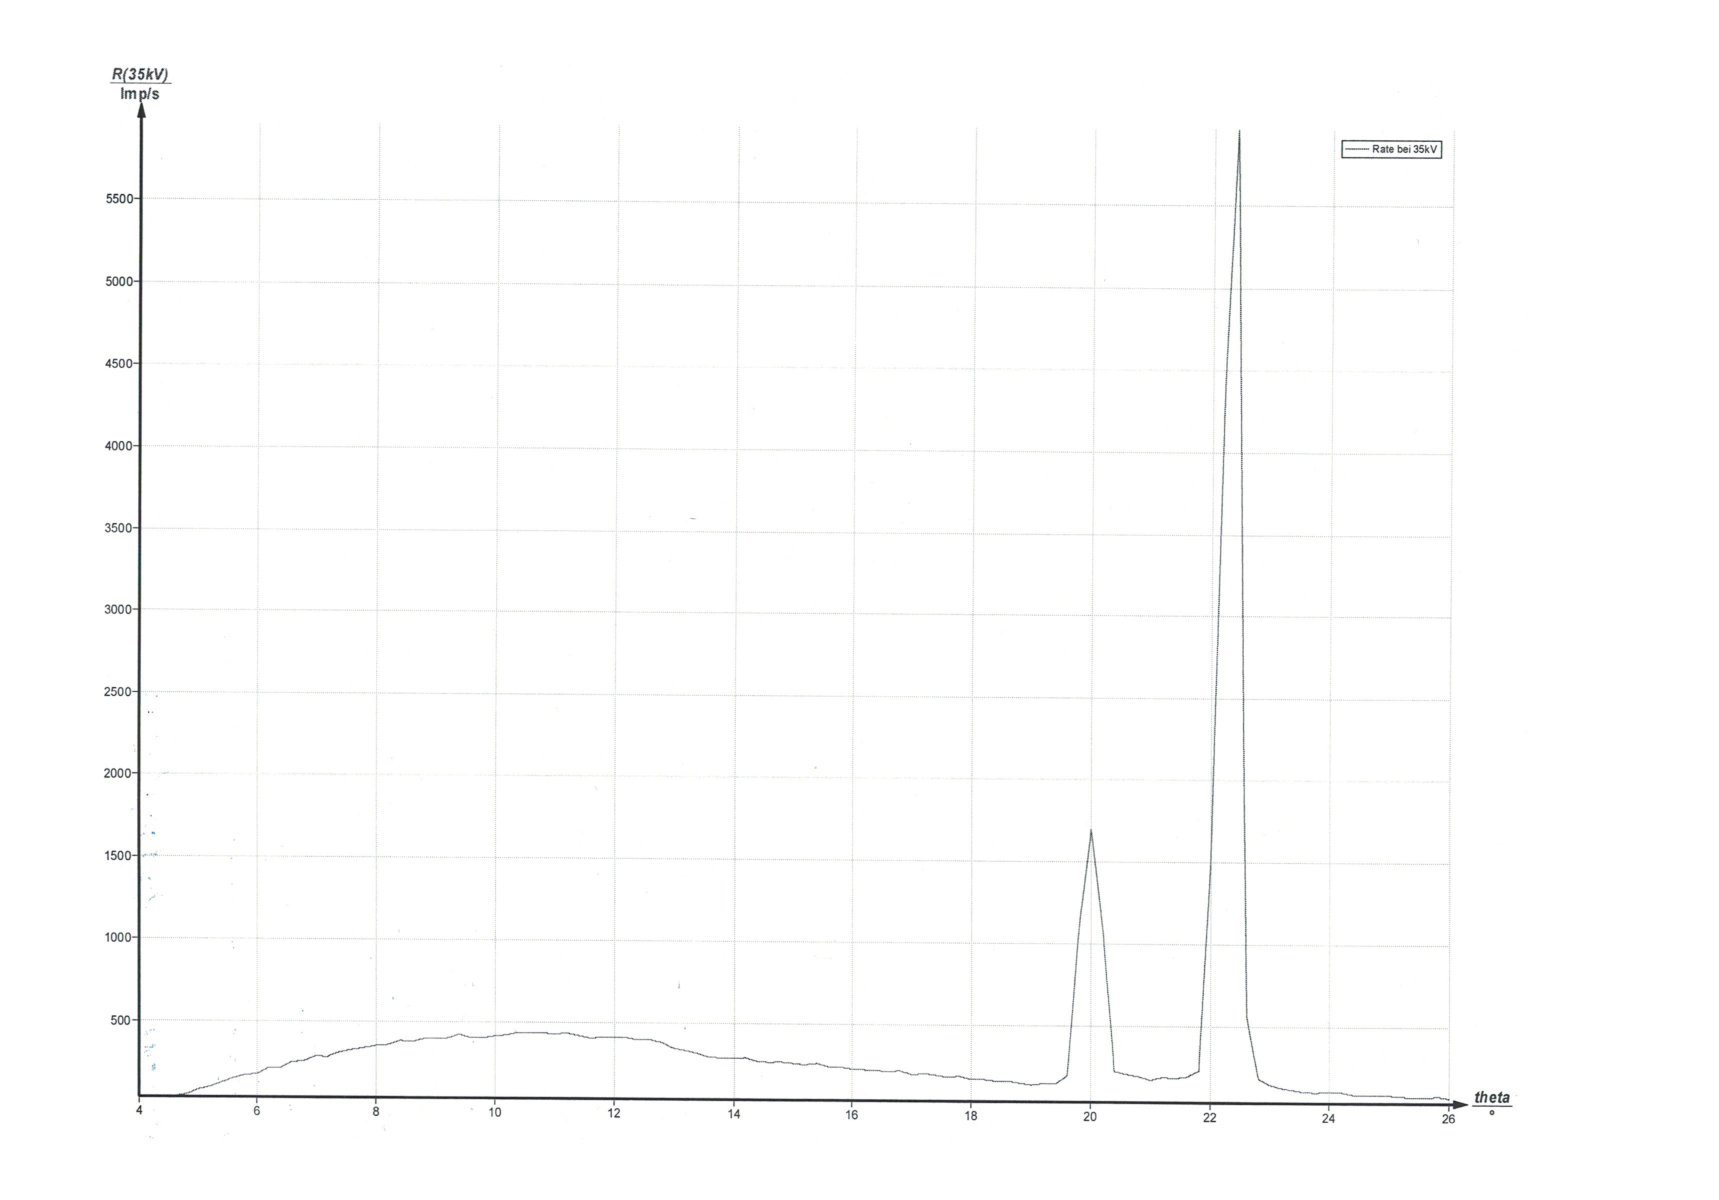
\includegraphics[width=\textwidth]{emissiongraph.pdf}
  \caption{Emissionsspektrum einer Cu-Röntgenröhre}
  \label{fig:emiss}
\end{figure}

\FloatBarrier

\subsection{Absorptionsspektrum}
Es wird vor das Geiger-Müller Zählrohr ein Material gesetzt was ein bestimmtes Absorptionsspektrum besitzt.
Dieses wird mit 0,1°-Schritten vermessen. Die Integrationszeit beträgt $\Delta t$=\SI{20}{s}
Da die Messung in der 2:1 Kopplung gemessen wurde müssen die Winkelangaben halbiert werden.
\subsubsection{Brom}
Mit den Gleichungen \ref{eqn:winkel} und  \ref{eqn:E} lässt sich die Absorptionsenergie und die Abschiermkonstante bestimmen.\\
 Die Ordnungszahl ist dabei
\begin{align*}
  Z=35.
\end{align*}
Der Winkel wird als $\SI{13,05\pm0,35}{°}$ gemessen.
Die Absorptionsenergie bertägt
\begin{align*}
  E_K=\SI{13,631\pm0,806}{keV}.
\end{align*}
Daraus ergiebt sich die Abschiermkonstante
\begin{align*}
  \sigma_{\text{K}}=\SI{3,347\pm0,922}{}.
\end{align*}
\begin{figure}[h!]
  \centering
  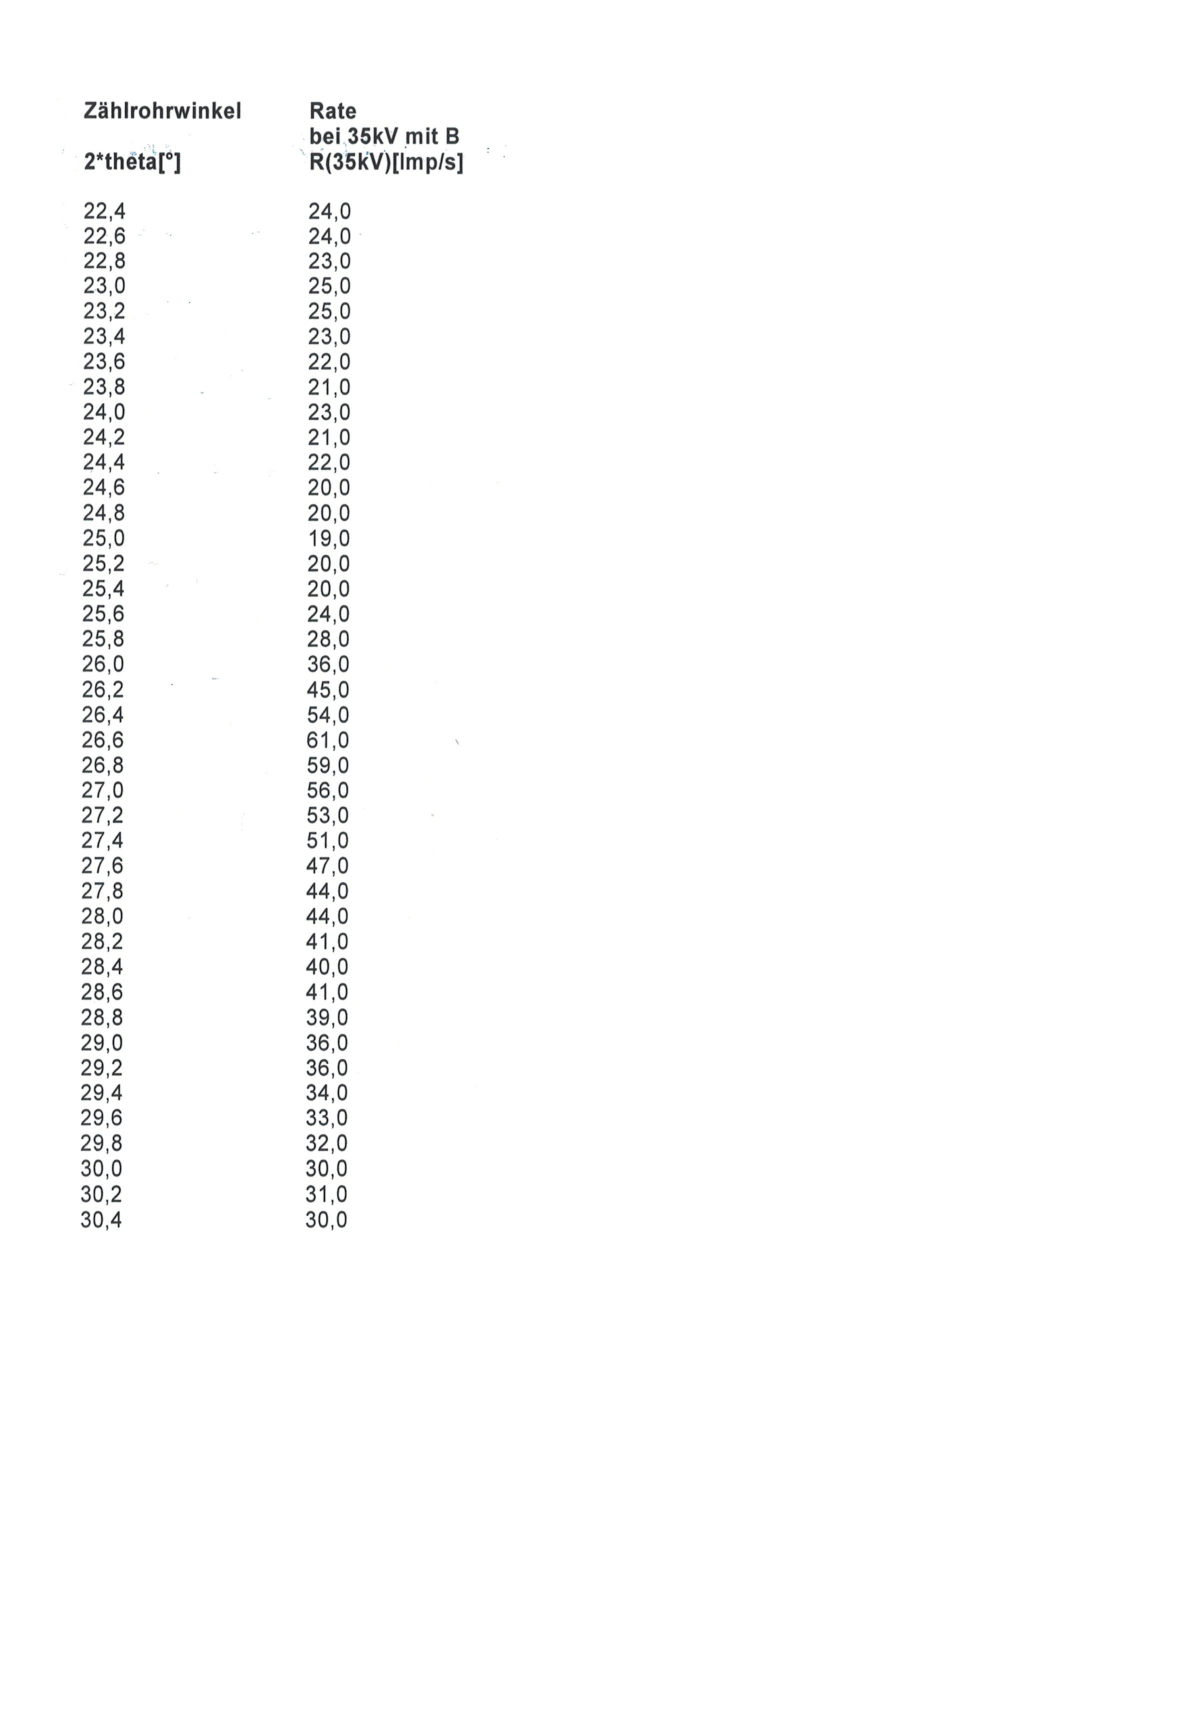
\includegraphics[width=0.4\textwidth]{bromtab.pdf}
  \caption{Absorptionsspektrum von Brom}
  \label{tab:brom}
\end{figure}
\begin{figure}[h!]
  \centering
  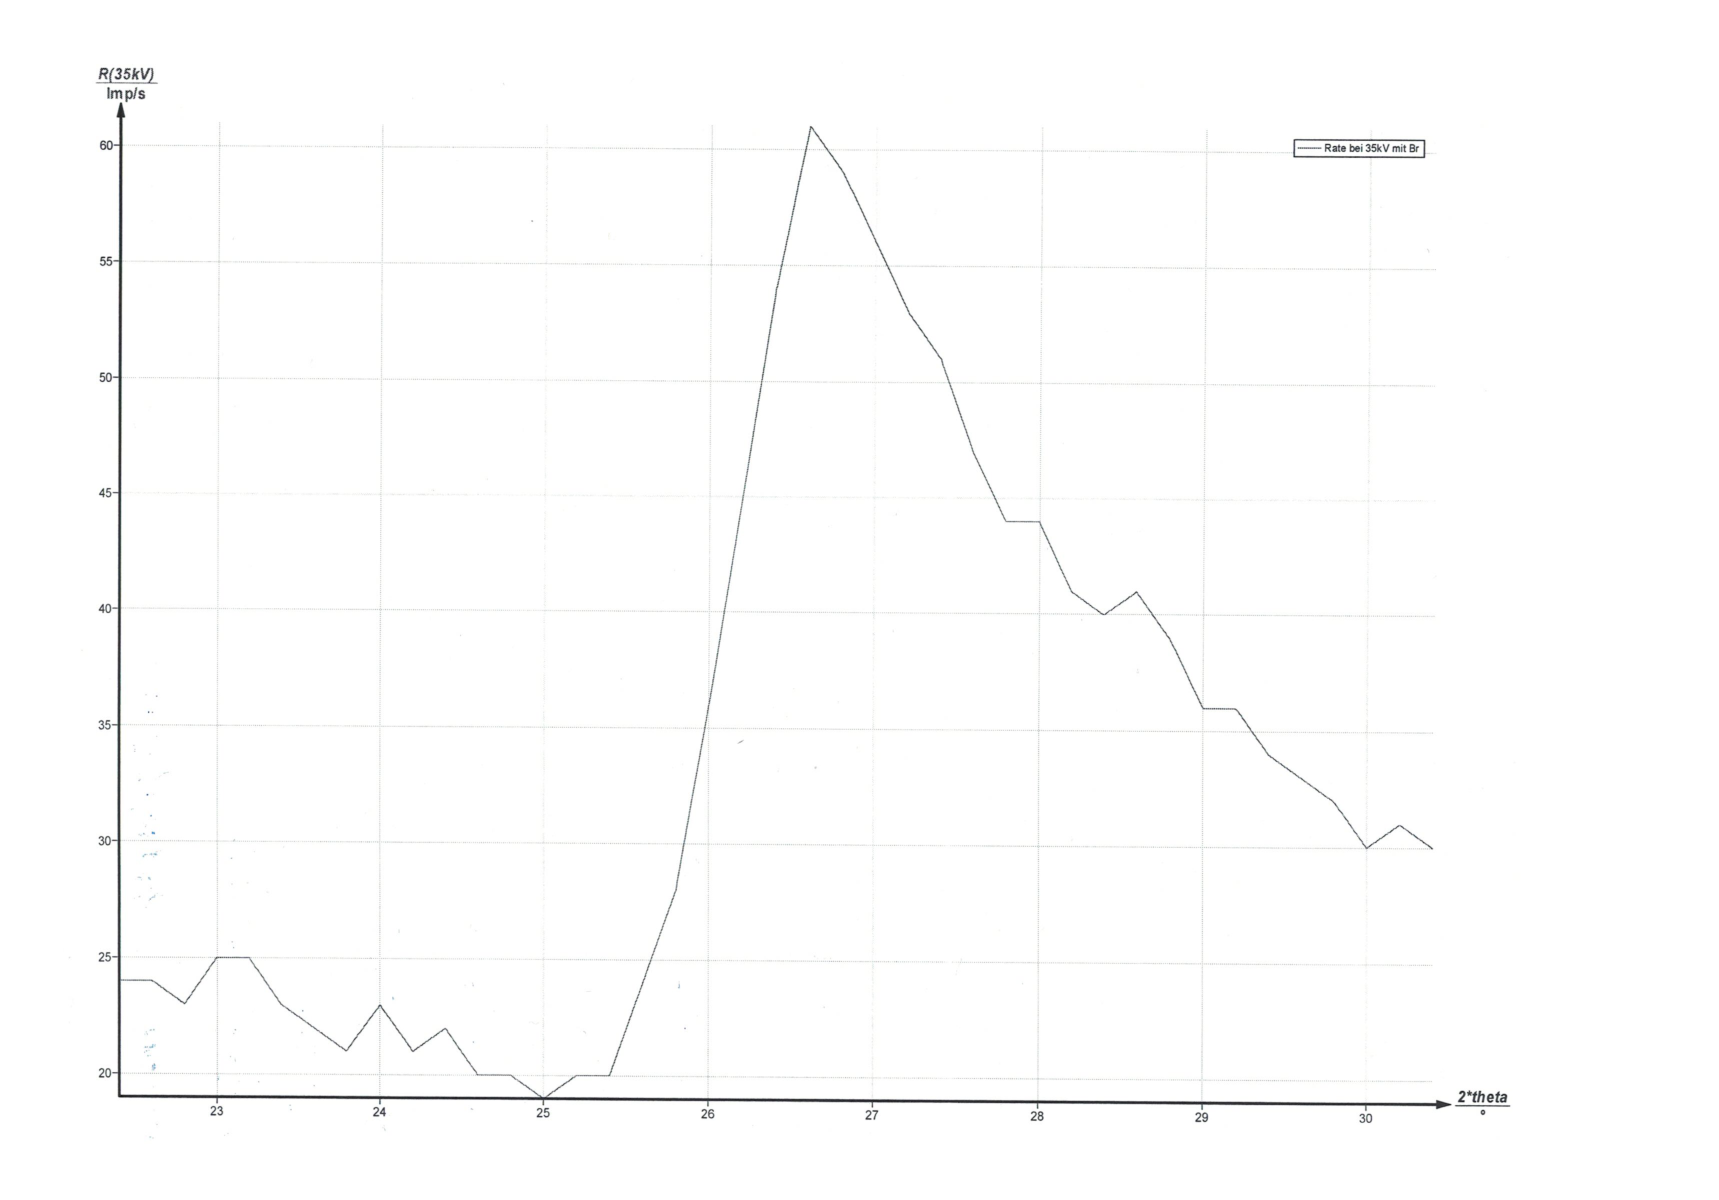
\includegraphics[width=\textwidth]{bromgraph.pdf}
  \caption{Absorptionsspektrum von Brom}
  \label{fig:brom}
\end{figure}
\FloatBarrier

\subsubsection{Strontium}
\begin{align*}
  Z&=38\\
  Winkel&=\SI{10,75\pm0,45}{°}\\
  E_K&=\SI{16,502\pm0,712}{keV}\\
  \sigma_{\text{K}}&=\SI{3,173\pm0,743}{}
\end{align*}

\begin{figure}[h!]
  \centering
  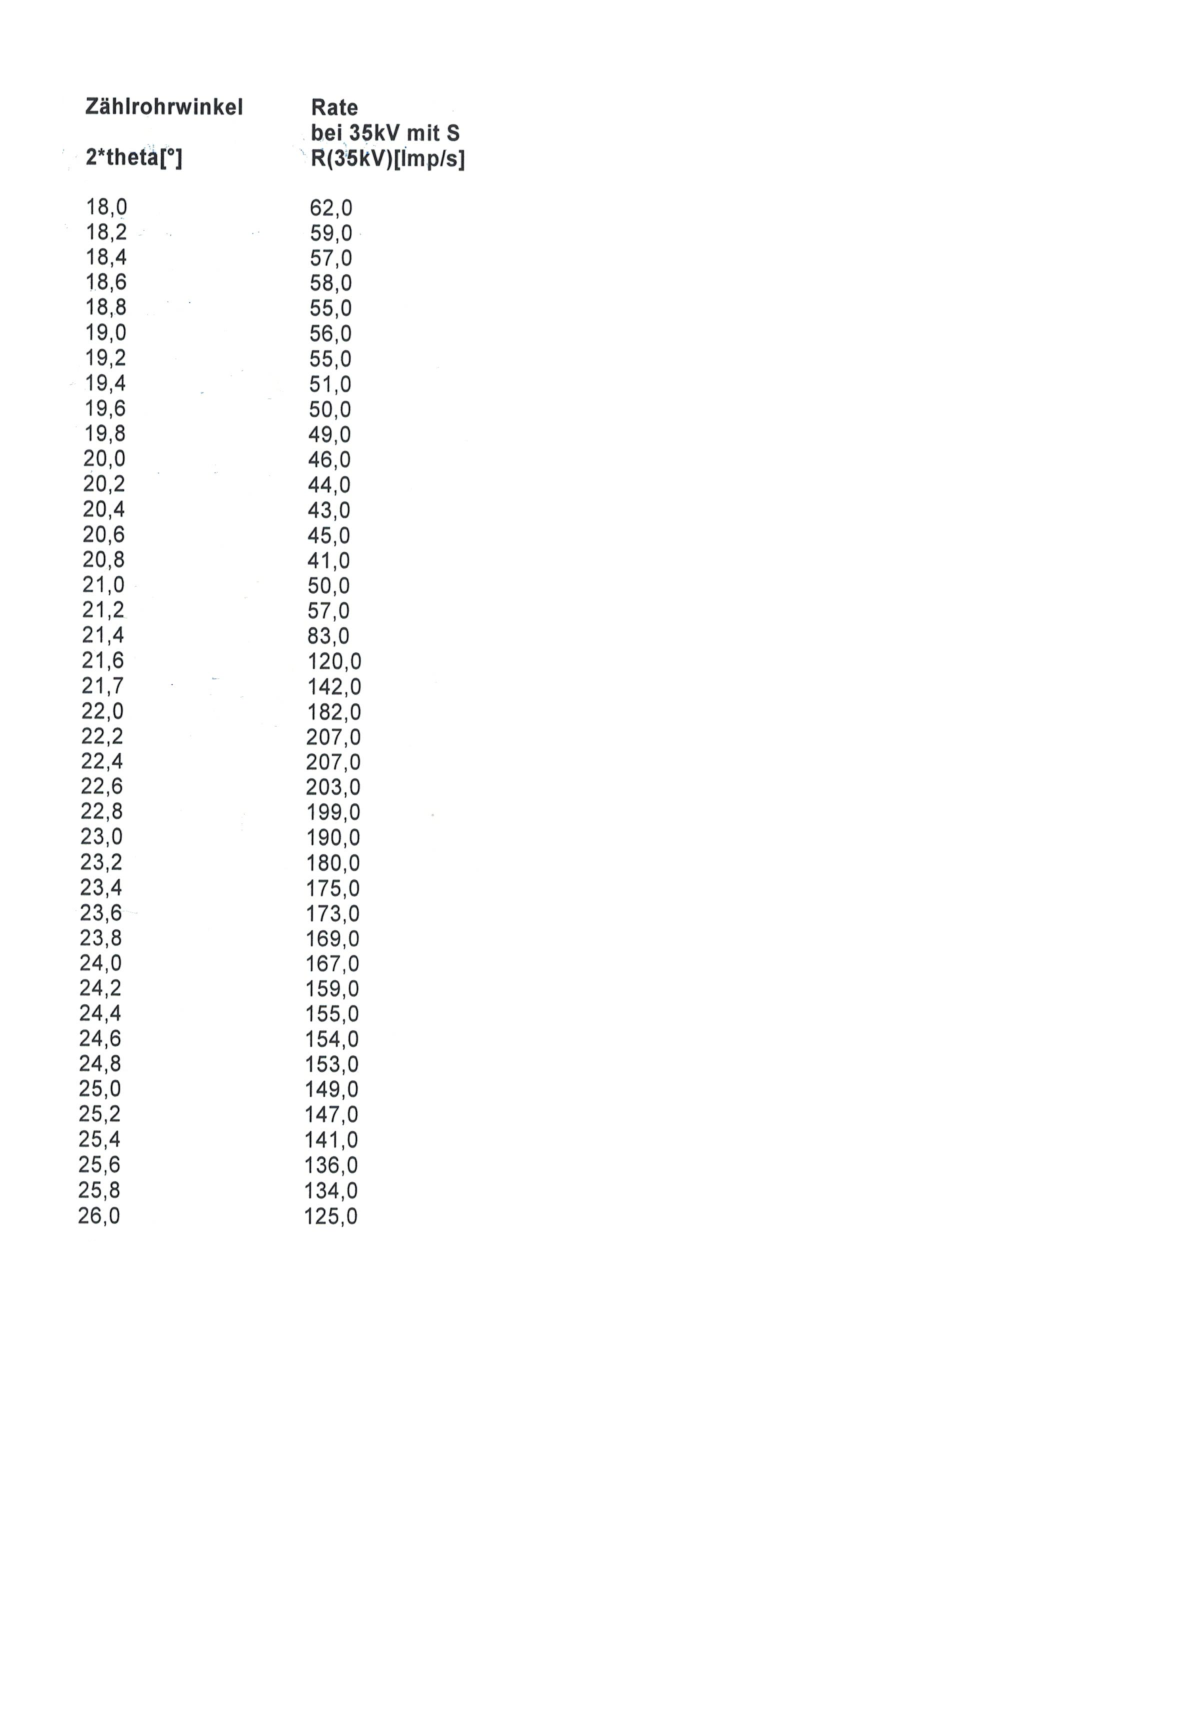
\includegraphics[width=0.4\textwidth]{strontiumtab.pdf}
  \caption{Absorptionsspektrum von Strontium}
  \label{tab:strontium}
\end{figure}
\begin{figure}[h!]
  \centering
  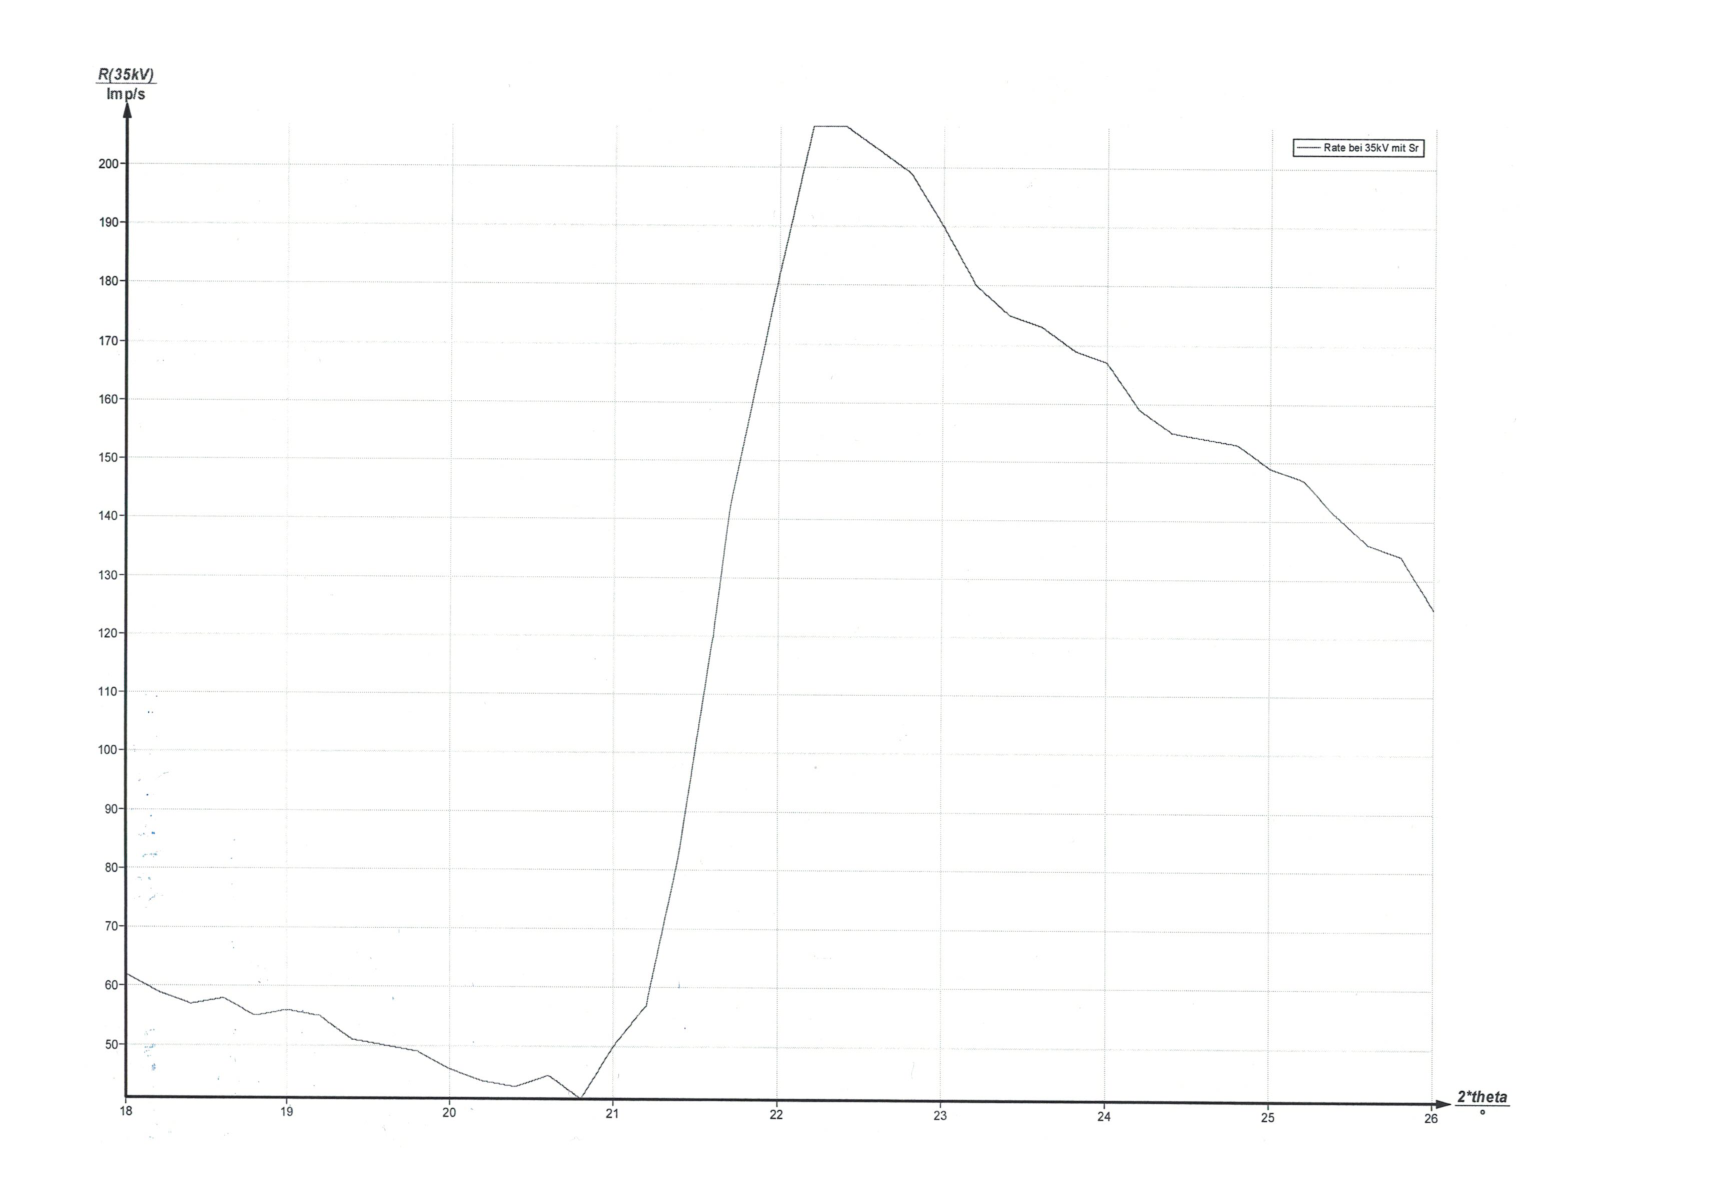
\includegraphics[width=\textwidth]{strontiumgraph.pdf}
  \caption{Absorptionsspektrum von Strontium}
  \label{fig:strontium}
\end{figure}
\FloatBarrier

\subsubsection{Zirkonium}
\begin{align*}
  Z&=40\\
  Winkel&=\SI{9,75\pm0,45}{°}\\
  E_K&=\SI{18,175\pm0,793}{keV}\\
  \sigma_{\text{K}}&=\SI{3,449\pm0,788}{}
\end{align*}

\begin{figure}[h!]
  \centering
  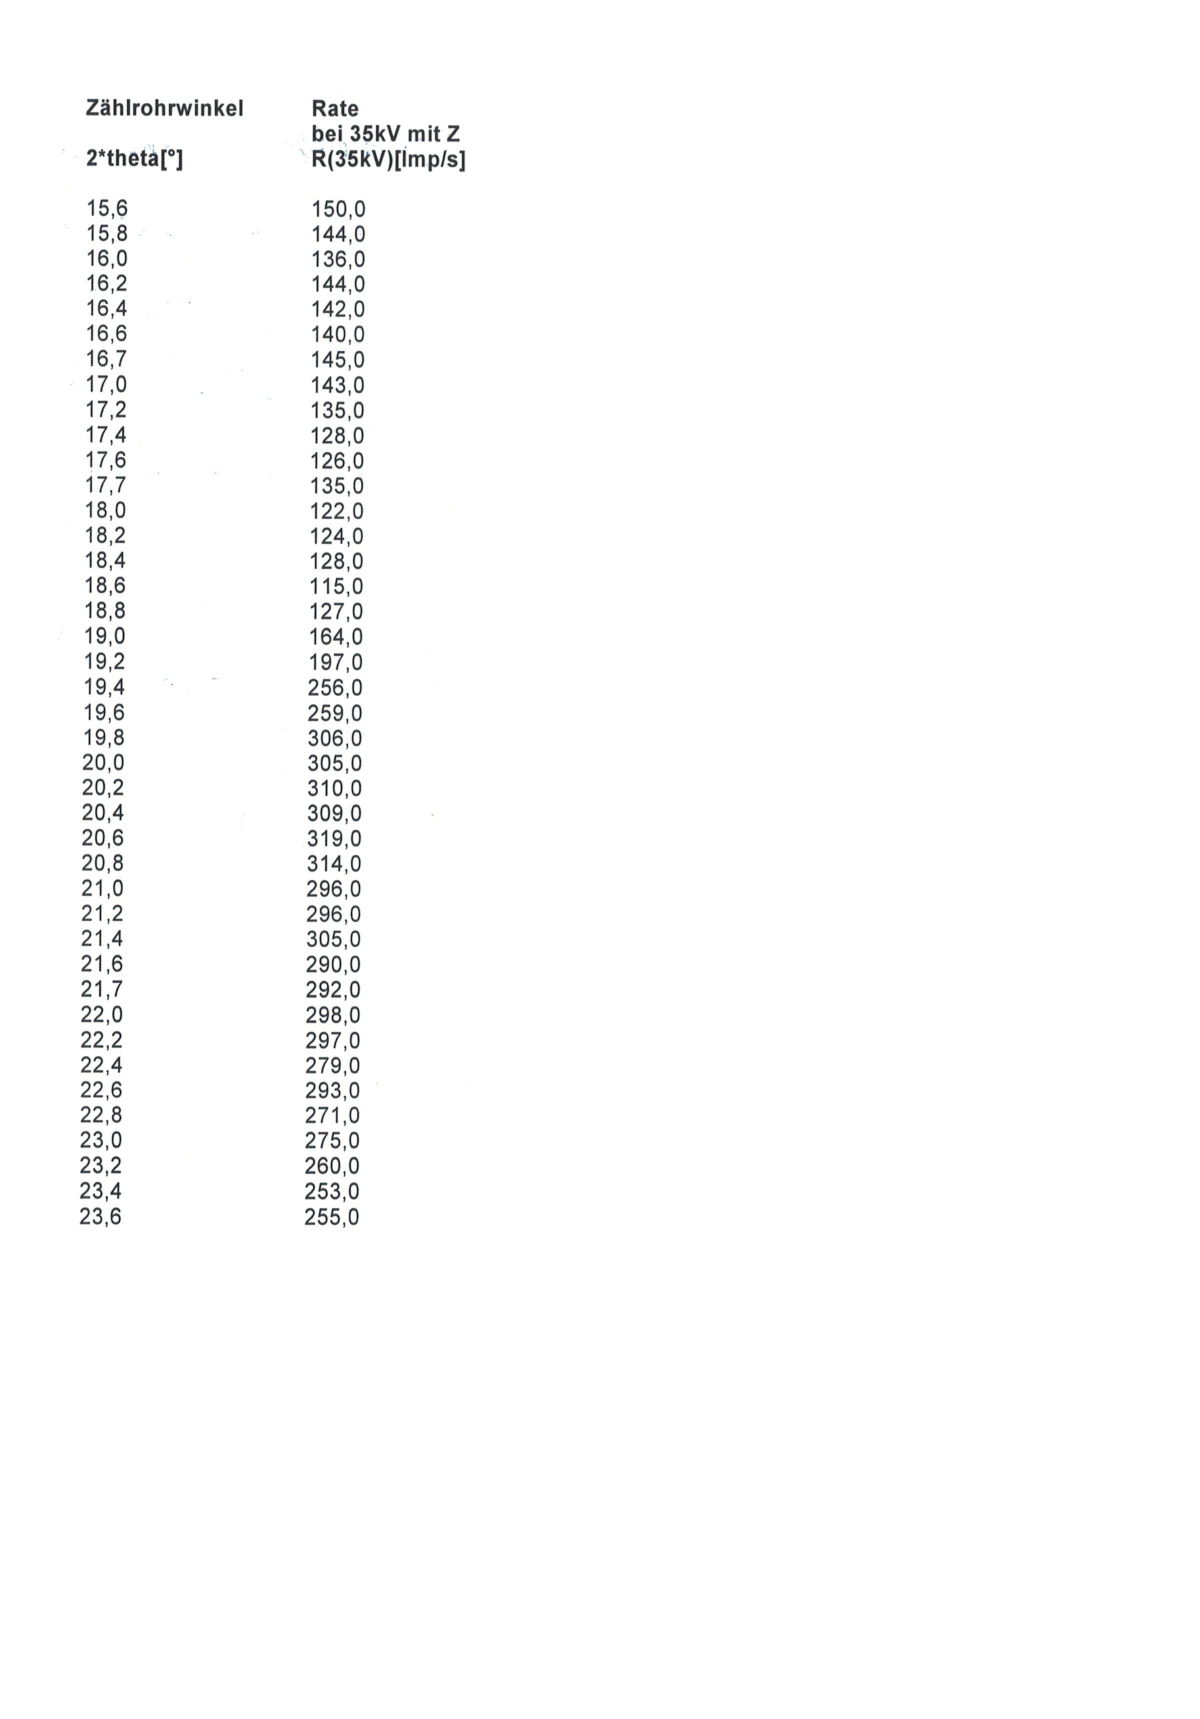
\includegraphics[width=0.4\textwidth]{zirkoniumtab.pdf}
  \caption{Absorptionsspektrum von Zirkonium}
  \label{tab:zirkonium}
\end{figure}
\begin{figure}[h!]
  \centering
  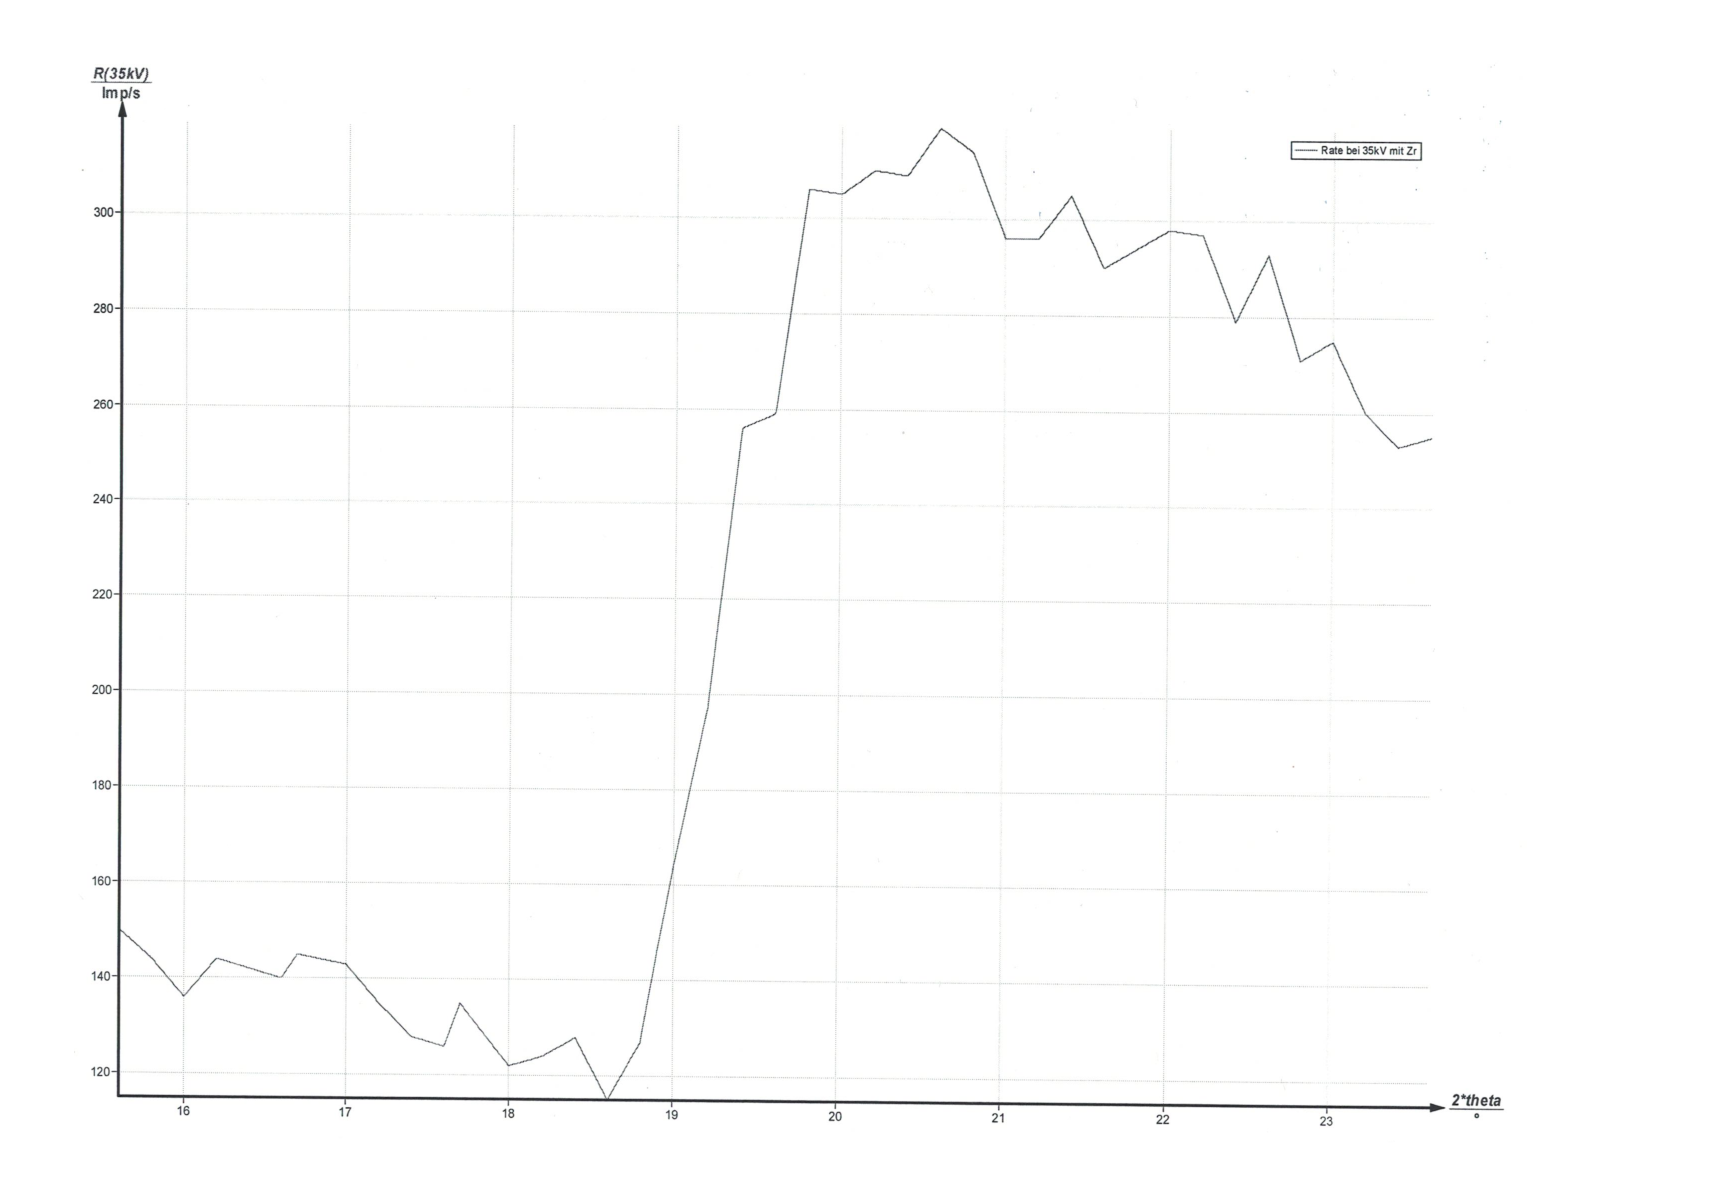
\includegraphics[width=\textwidth]{zirkoniumgraph.pdf}
  \caption{Absorptionsspektrum von Zirkonium}
  \label{fig:zirkonium}
\end{figure}
\FloatBarrier
\subsection{Moselysches-Gesetz}
Mit den Energiewerten für Zirkonium, Strontium und Brom und deren Ortnungszahlen läst sich die  Rydbergkonstante bestimmen.
Dazu wird die Wurzel der Energie gegen die Ordnungszahl Z aufgetragen.
Mit einer von Python errechneten Ausgleichsgraden werden folgende werte bestimmt.
\begin{align*}
  y&=mx+b\\
  m&=(3,753\pm2,874\cdot10^{-4})\si{\sqrt{eV}}\\
  b&=(-12,085\pm0,141)\si{\sqrt{eV}}
\end{align*}
Mit den Gleichungen
\begin{align*}
  E_{\text{Ry}}&=m^2\\
  \Delta E_{\text{Ry}}&=\sqrt{(2\cdot m)^2\cdot\Delta m}
\end{align*}
lässt sich die Rydbergkonstante und ihr Fehler, mit hilfe der Gaußschen Fehlerfortpflanzung, bestimmen.
\begin{align*}
  E_{\text{Ry}}=\SI{14,08\pm0,12}{eV}
\end{align*}
\begin{figure}[h!]
  \centering
  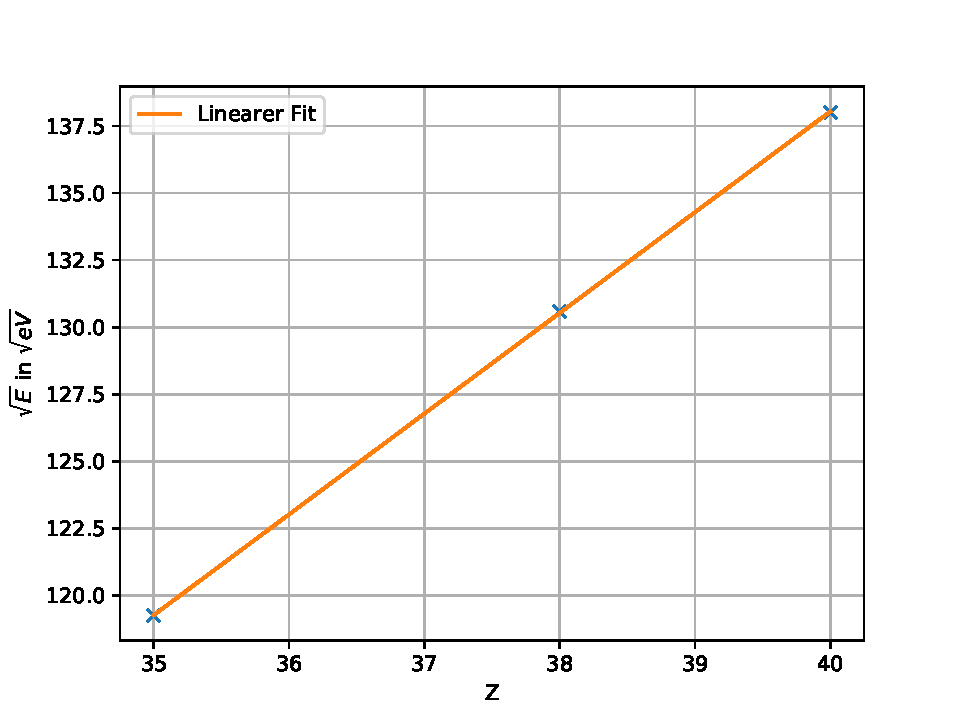
\includegraphics[width=0.8\textwidth]{ZgE.pdf}
  \caption{$\sqrt{E}$-Z Diagramm}
  \label{fig:ZgE}
\end{figure}
\FloatBarrier

\subsubsection{Quecksilber}
Quecksilber hat eine hohe Ordnungszahl, daher lassen sich bei Quecksilber die Parameter für die L-Kante bestimmen.
\begin{align*}
  Z&=80\\
  Winkel_{L2}&=\SI{14,6\pm0,1}{°}       &Winkel_{L3}&=\SI{14\pm0,1}{°}\\
  E_{L2}&=\SI{12,211\pm0,081}{keV}      &E_{L3}&=\SI{12,723\pm0,088}{keV}\\
  \sigma_{\text{L2}}&=\SI{50\pm0,05}{}  &\sigma_{\text{L3}}&=\SI{49,419\pm0,105}{}
\end{align*}
Die Energiedifferenz beträgt:
\begin{align*}
  \Delta E=\SI{12,723}{keV}-\SI{12,211}{keV}=\SI{0,512}{keV}
\end{align*}
Daraus läst sich mit der Formel \ref{eqn:sigL} die Abschirmkonstante $\sigma_{\text{L}}$ berechnen.
\begin{align*}
  \sigma_{\text{L}}=23,624
\end{align*}
\begin{figure}[h!]
  \centering
  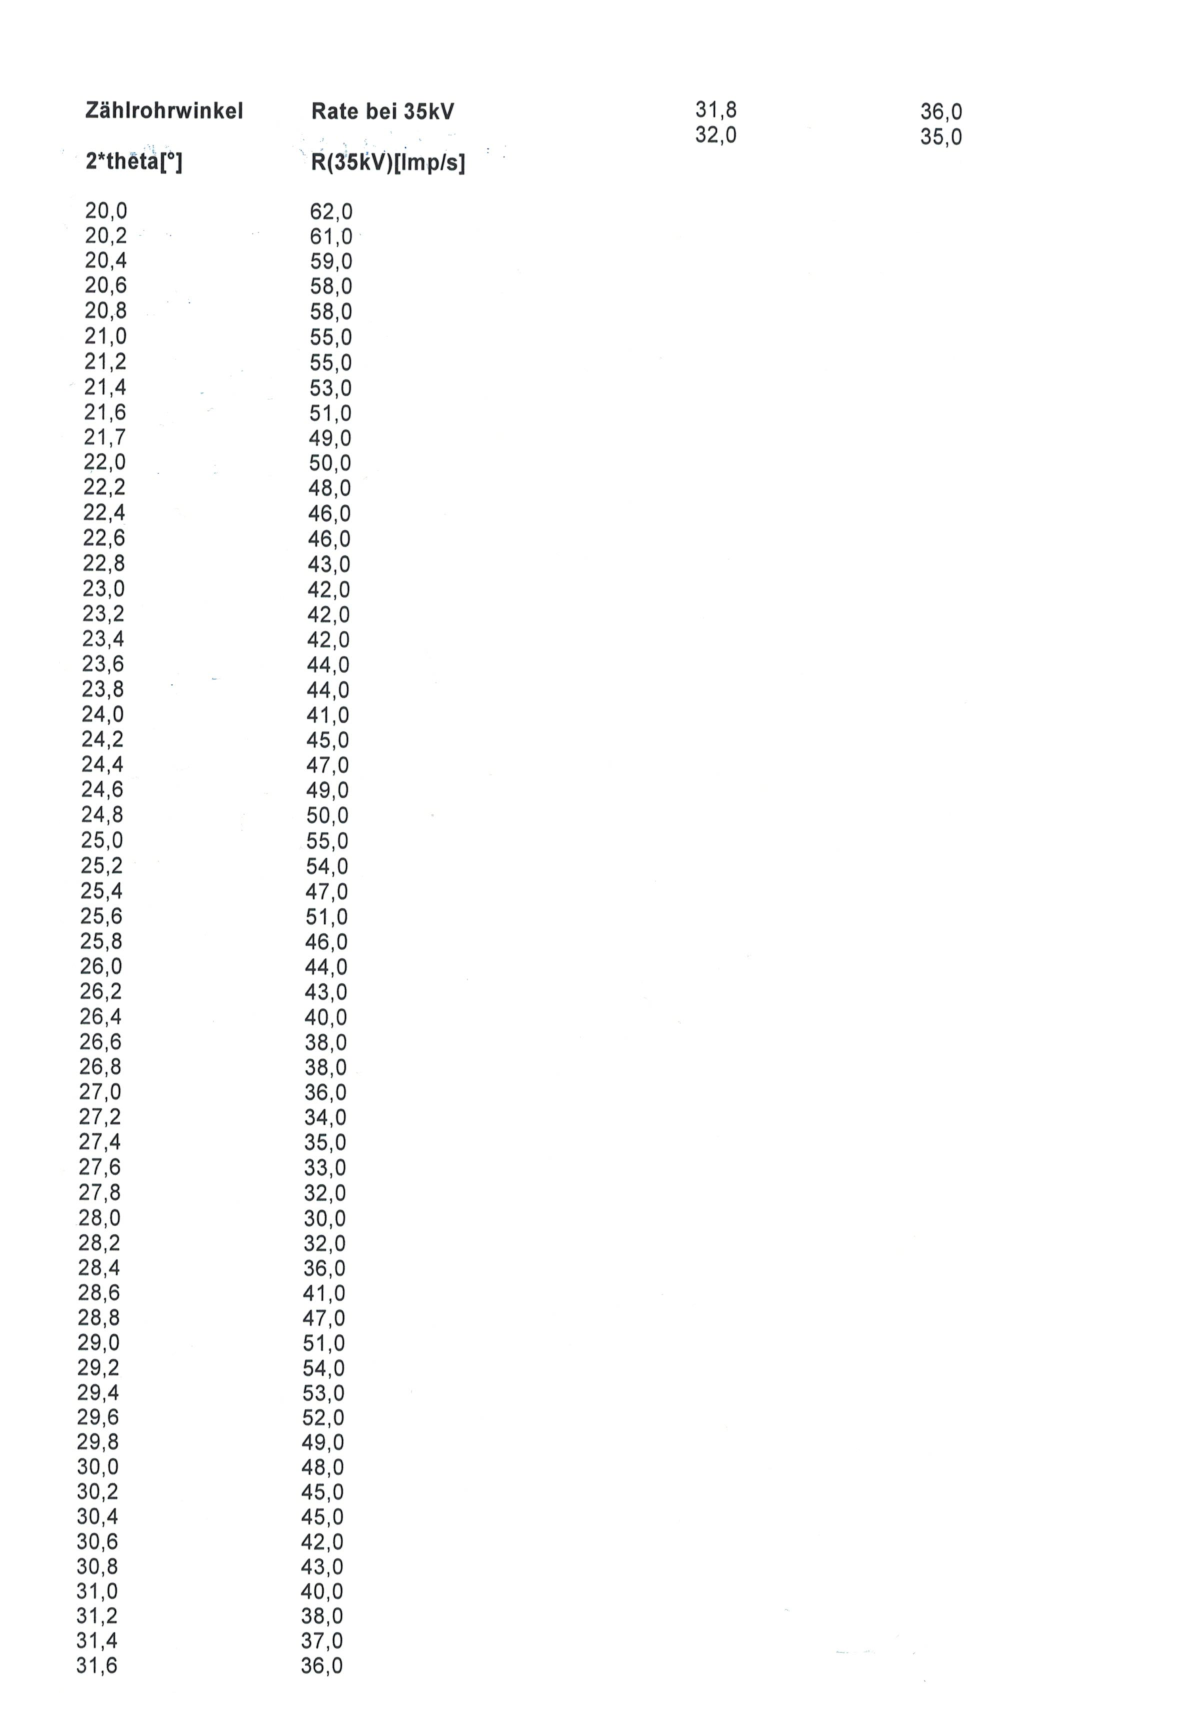
\includegraphics[width=0.8\textwidth]{quecksilbertab.pdf}
  \caption{Absorptionsspektrum von Quecksilber}
  \label{tab:quecksilber}
\end{figure}
\begin{figure}[h!]
  \centering
  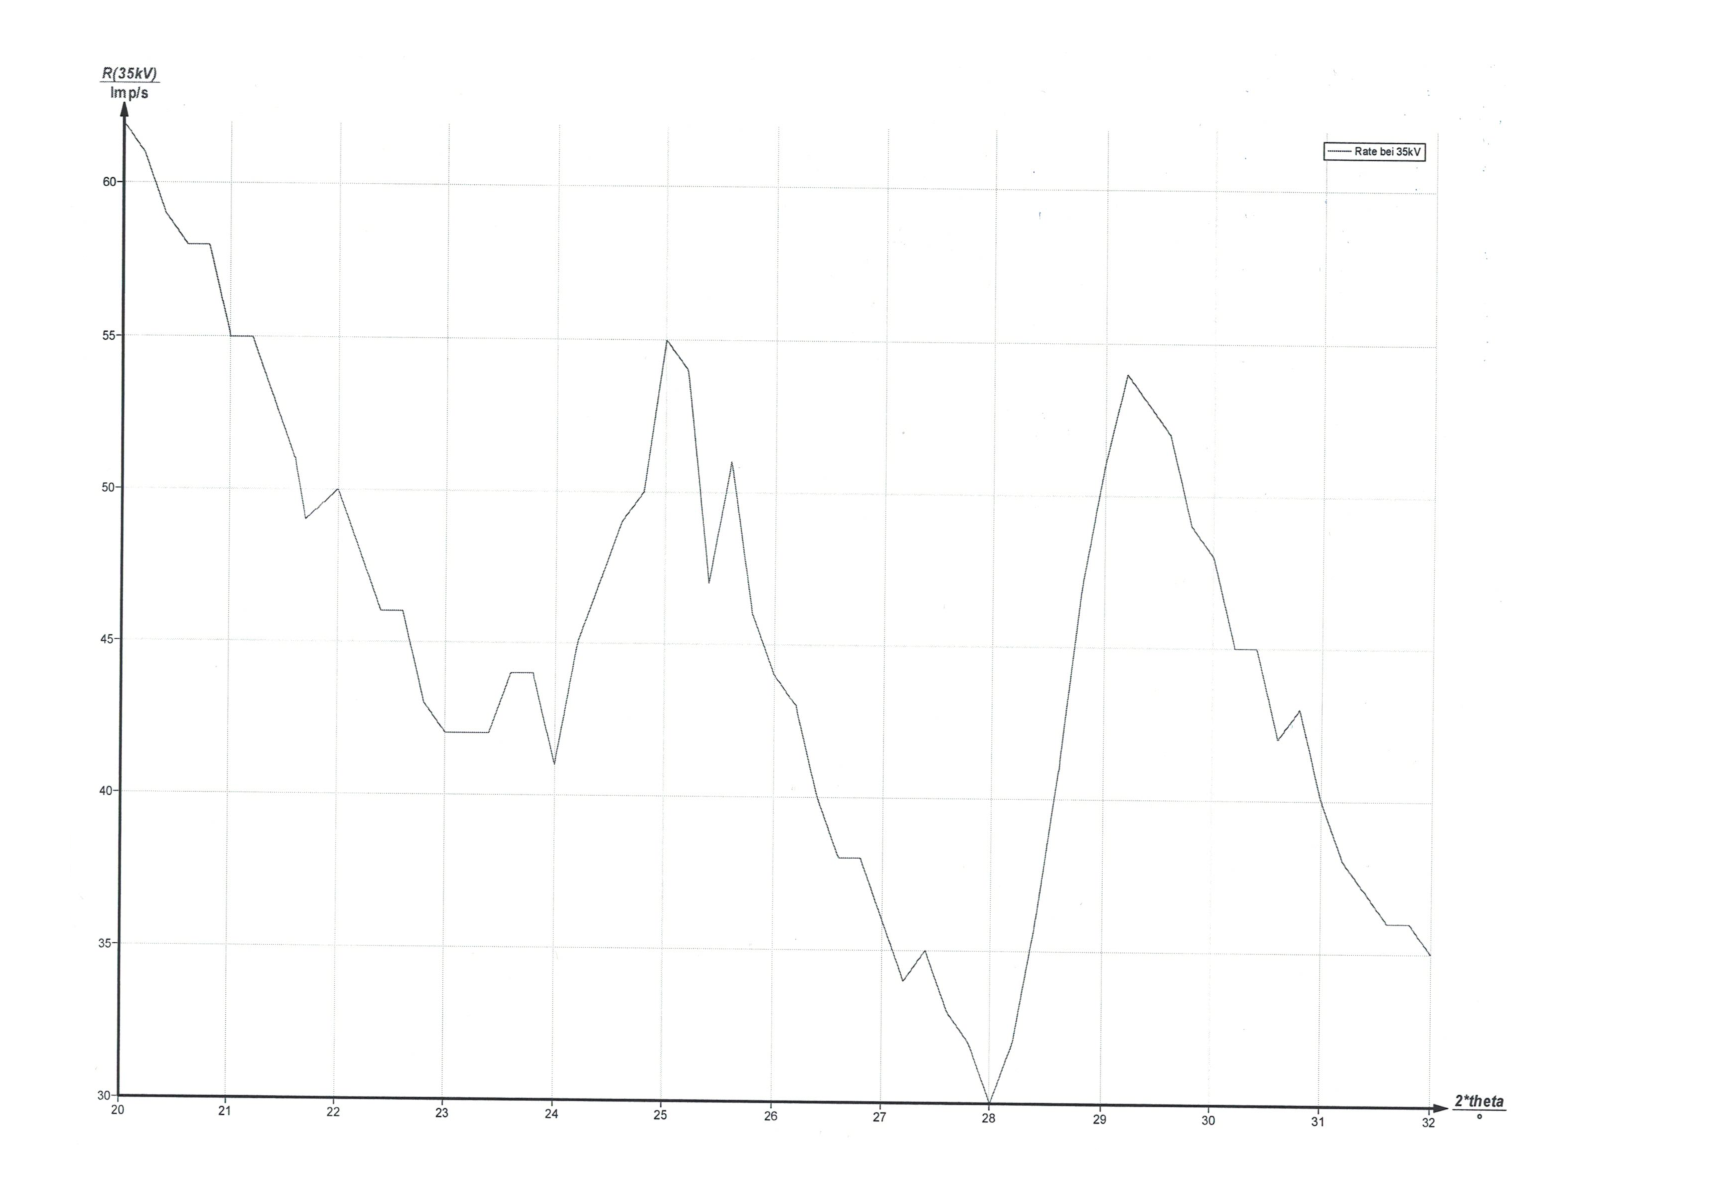
\includegraphics[width=\textwidth]{quecksilbergraph.pdf}
  \caption{Absorptionsspektrum von Quecksilber}
  \label{fig:quecksilber}
\end{figure}
